
\documentclass{article}

\usepackage{graphicx}
\usepackage{hyperref}
\usepackage{biblatex}
\addbibresource{Readme.bib}
\usepackage{minted}
\newmintinline[coq]{coq}{}
\newmintinline[rust]{rust}{}

\renewcommand*{\thefootnote}{\fnsymbol{footnote}}

\author{
     Sidney Congard
\and Son Ho
\and Aymeric Fromherz
}
\title{Aeneas Coq backend}

\begin{document}

\maketitle

Aeneas (\cite{Aeneas}) is a framework translating a subset of safe Rust programs into pure lambda-calculus, which can then be embedded in various proof assistants. This article describes the framework built to welcome those translations in Coq and to  verify them easily.

\medskip

The first part (\nameref{sec:Translation}) presents the translated code, by showing how it can fit inside Coq type system while remaining lightweight and faithful to the original code.

Then, the second part (\nameref{sec:Lemmas}) presents the theorems established on the translation basic building blocks : their choice determines how we can reason on translated programs.

The third part (\nameref{sec:Tactics}) is due to the fact that lemmas alone only enable low-level, manuel reasoning. It introduces high-level tactics to automatize basic rules and to smooth up the specificities introduced by the translation.

The two last parts detail choices and limitations from the framework. In \nameref{sec:Tradeoffs}, those are choices of design, contrarily to issues listed in \nameref{sec:Implementation} which should disappear with more work.

\section{Translation}
\label{sec:Translation}

Most Rust functions can panic, due to arithmetic overflow, out of bounds access, ... In the functional translation, this is reflected by a result monad which may return an error containing no information. Moreover, because Coq is as total programming language, a fuel\footnote{This is a common technique to write the function with structural recursion, by matching on the fuel (a natural number) argument.} parameter is passed to recursive functions. This allows to do partial correctness as well.

For those reasons, the output type of translated functions is wrapped into a result monad yielding either :
\begin{itemize}
    \item The value in case of success.
    \item A failure matching a panic.
    \item An "out of fuel" error.
\end{itemize}

\medskip

Most supported types are translated straightforwardly into inductive types. However, scalars and vectors benefit instead of a builtin representation to ease their manipulation.

Scalars are translated into dependent pairs : they are represented with Z and associated with bounds between their minimal and maximal value. Similarly, vectors and translated to lists associated with a bound on their size. Representing integers with Z is useful to be able to leverage the "lia" tactic to prove arithmetic facts efficiently. It also help keeping decent performances (compared to e.g. nat).

\medskip

To give a small example, here is a recursive function behaving like the identity function :

\begin{minted}{Rust}
// A complicated way to return 0.
fn usize_identity(s: usize) -> usize {
    if (s == 0) {
        0
    } else {
        usize_identity(s - 1) + 1
    }
}
\end{minted}

% TODO Use Aeneas to get the exact translation.
This is how the Coq backed translates it :

\begin{minted}{Coq}
Fixpoint usize_identity (fuel: nat) (s: usize) : result usize :=
(* Handles total recursion with the fuel. *)
match fuel with
| 0%nat => Fail_ OutOfFuel
| S fuel =>
    if (s s= 0%usize) then Return 0%usize else
    (* Arithmetic operations are monadic. *)
    x <- usize_sub s (1%usize);
    y <- usize_identity fuel x;
    usize_add y (1%usize)
end.
\end{minted}

% TODO Check this claim with Son.
This backend supports any translation from Aeneas. To explore in more details which programs are supported and how they are translated (especially in presence of borrowing) by Aeneas, we refer to \cite{Aeneas}.

\section{Lemmas}
\label{sec:Lemmas}

Now that our Rust program is represented in Coq, we want to prove things about it. For that, the backend comes with lemmas to cover the result monad and the primitive types (mainly scalars and vectors).

\medskip

Because dependent types can be heavy to manipulate directly, lemmas on scalars and vectors reason instead on their projections to their value and its bounds. In particular, proof irrelevance is imported to equate them on those projections.

Fallible operations $f(x)$ (such as "scalar\_add") are mainly handled by "monadic lemmas", a class of lemmas in the following shape :

$Preconditions(x) \rightarrow \exists y:T, f(x) = Return(y) \wedge Postconditions(x, y)$.

\begin{minted}{Coq}
(* The monadic lemma for scalar addition. *)
Lemma S_add_bounded {ty} (n m: scalar ty) :
    scalar_min ty <= (to_Z n) + (to_Z m) <= scalar_max ty ->
    exists x, scalar_add n m = Return x
     /\ to_Z x = (to_Z n) + (to_Z m).
\end{minted}

A variant for partial correctness can be done by asserting that there are no "out of fuel" error in preconditions :

\begin{minted}{Coq}
(* A monadic lemma for our "usize_identity" function above. *)
Lemma usize_identity_shape fuel s :
    usize_identity fuel s != Fail_ OutOfFuel ->
    exists v, usize_identity fuel s = Return v
        /\ to_Z s = to_Z v.
\end{minted}

Often, lemmas of this shape are more convenient to use, but less convenient to prove used compare to those with written with a "match" instead :

\begin{minted}{Coq}
(* Easier to prove. *)
Lemma usize_identity_shape fuel s :
  match usize_identity fuel s with
  | Return v => to_Z s = to_Z v
  | Fail_ OutOfFuel => True
  | Fail_ Failure   => False
  end.
\end{minted}

For this, lemmas assure that existential formulations and those with a "match" are equivalent. They exist for both the partial correctness and total correctness variants.

\medskip

While the main properties are proven by monadic lemmas, other lemmas are given to e.g. simplify monadic expressions exclusively.

\section{Tactics}
\label{sec:Tactics}

Even equipped with those lemmas, the verification of programs such as "usize\_identity" remains tedious : too much time must be passed by using monadic only to peel away the monadic notation.

For this reason, one high-level tactic "aeProgress" is provided, built on three other tactics to automatize most of the basic reasoning concerning arithmetic and monadic operations (on scalars, vectors or used-provided structures). They are based on a rewrite hint database and three typeclasses to extend them with new user-provided lemmas :

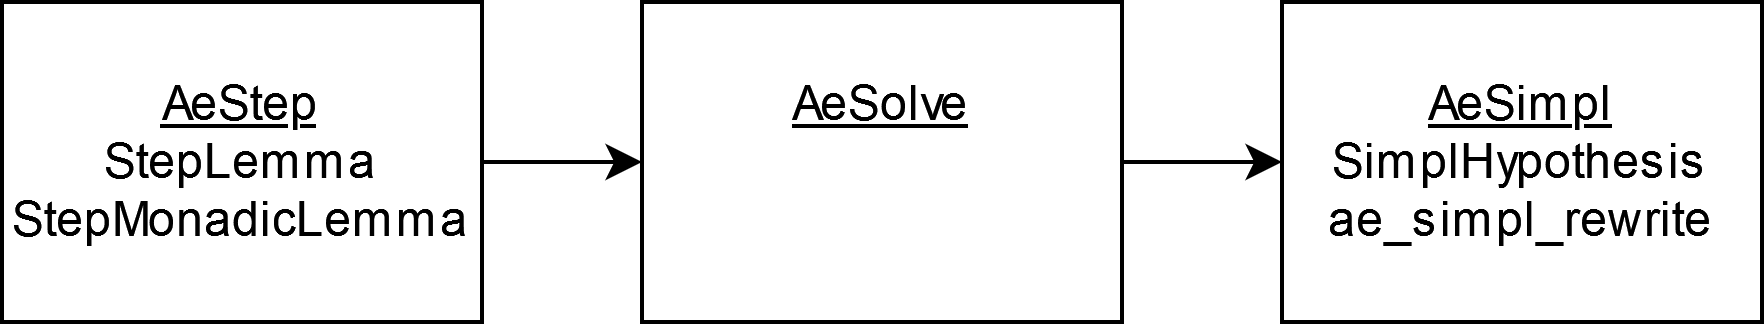
\includegraphics[width=0.9\textwidth]{Readme-tactics.png}

\begin{itemize}
    \item "aeSimpl" uniformizes the context with a "SimplHypothesis" typeclass providing hypotheses to add in the context. It then simplify everything and apply the directed equations recorded in the "ae\_simpl\_rewrite" hint database.
    \item "aeSolve" tries to solve the current goal by simplifying it with "aeSimpl" then applying on it the generic tactic "easy", otherwise "lia".
    \item "aeStep" advances on the current goal : it visits the goal until it gets stuck on a blocking term. Then, it lookups a lemma on the term from the typeclasses "StepMonadicLemma" (accepting monadic lemmas) or else "StepLemma" (accepting any lemma) to add to the context before destructing the term. Finally, it tries to satisfy lemmas preconditions with "aeSolve".
\end{itemize}

\medskip

There are also small tactics to do induction on usize as nat and to simplify ("siphon") the fuel.

Put together, here is a proof for our monadic lemma on "usize\_identity" :

\begin{minted}{Coq}
Lemma usize_identity_shape fuel s :
  match usize_identity fuel s with
  | Return v => to_Z s = to_Z v
  | Fail_ OutOfFuel => True
  | Fail_ Failure   => False
  end.
Proof.
revert fuel.
induction_usize_to_nat s as S;
intro fuel;
(* Unfolds "usize_identity_shape". *)
siphon fuel;
(* Advances on the scalar comparison. *)
aeStep b;
aeSimpl;
try aeSolve.

(* Successor case: *)

(* Advances on the incremented value. *)
aeStep r.
aeSimpl.

(* IH argument *)
assert (B: usize_to_nat r = S). 1: {
  cut (Z.of_nat (usize_to_nat r) = Z.of_nat S).
  - intuition.
  - aeSolve.
}
assert (H := IHS r B fuel).
destruct (usize_identity fuel r). 2: aeSolve.
aeSimpl.

(* Advances on the decremented value. *)
aeStep r0.
aeSolve.
Qed.
\end{minted}

Finally, a high-level tactic "aeProgress" combines the three tactics above by applying as much as possible "aeStep", "aeSimpl" and "aeSolve". The proof above can then be further simplified :

\begin{minted}{Coq}
revert fuel.
induction_usize_to_nat s as S;
intro fuel;
siphon fuel;
aeProgress b r.

(* IH argument *)
assert (B: usize_to_nat r = S). 1: {
    cut (Z.of_nat (usize_to_nat r) = Z.of_nat S).
    - intuition.
    - aeSolve.
}
assert (H := IHS r B fuel).
destruct (usize_identity fuel r);
aeProgress.
Qed.
\end{minted}

The tactic "aeProgressOnce" can be useful as well, as it acts like a more convenient "aeStep" : it also calls "aeSimpl" first and calls "aeSolve" if "aeStep" didn't succeed.

\section{Tradeoffs}
\label{sec:Tradeoffs}

Here are the main opinionated choices done for this framework.

% tactics style
\medskip

As explained in previous sections, lemmas only establish properties on scalars and vector underlying values. This makes them more verbose, but we need fewer of them (especially for arithmetic) and they are more uniform, so better fit for automation.

The framework was first developed with lemmas on scalars and vectors, resulting a proliferation of lemmas which is not only harder to produce and maintain, but also painful to use by looking up which precise lemma is needed at each step.

% ltac
\medskip

Tactics are written with Ltac. Ltac2 was considered but lacking in documentation, sometimes without direct alternatives to Ltac features. With adequate expertise, Ltac2 may be a good choice for the long run : it claims major gains in performances and corrects common issues with Ltac. Notably, it provides non-backtracking (i.e. fatal) errors, which should be useful to debug and signal internal errors from the framework, otherwise difficult to recognize as an user.

% simpl
\medskip

The "aeSimpl" tactic calls "simpl in *". This liberal use of simplification is done to improve the efficiency of tactics : the alternative ways to allow the user to re-introduce more local calls to "simpl" were too heavy or not covering all wanted cases. For example, "lia" do not recognize scalar constants like $to\_Z \; 42\%usize$, blocking proof automation.

% unfolding
\medskip

Because Coq doesn't support one-step reduction (e.g. "cbv delta1"), we use "simpl" instead to unfold typeclasses instances, which may trigger too much simplifications. This is needed to clear the instance from the context in the tactics.

One alternative strategy to unfold instances was to use "hnf" instead of "simpl", but it resulted in unwanted simplifications at different places, e.g. :
\begin{itemize}
    \item $x \ne Fail\_ OutOfFuel$ is unfolded to $x = Fail\_ OutOfFuel \rightarrow False$, so tactics and lemmas handling partial correction must be adjusted.
    \item The comparison of Z numbers $x < y$ is unfolded into $(x ?= y) = Lt$. It breaks proof automation because the "lia" tactic only takes the first expression into account : we must refold manually the expression.
\end{itemize}

The main consequence of the widespread use of "simpl" is that tactics may not work as excepted on a goal which may be further simplified or with typeclass instances not stable enough under "simpl". For example, when calling "aeStep" on a blocking term $x$ which simplifies to $y$, the looked up lemma may mention $x$ but $y$ after its simplification. Then, when "aeStep" destructs $x$, the lemma is not updated : we loose information and the goal may not be provable anymore.

We could insert a simplification before "aeStep" but prefer giving the choice to the user, as "aeProgressOnce" should be preferred by default for high-level reasoning.

\section{Implementation}
\label{sec:Implementation}

This section details the main limitations due to the implementation state. They should be addressable with enough effort.

% files
\medskip

The current implementation is split in two files : definitions are contained in "Primitives.v" while lemmas and tactics are in "Primitives\_Ext.v" along basic examples. All identifiers but examples live in the same scope for each file : this exposes tactics or lemmas that we may want to hide.

% injection
\medskip

Because "aeStep" progresses by destructing blocking terms, it does not progress by applying lemmas to the goal (which works on the whole term). That limits automation, which can benefit from another typeclass used to lookup and apply lemmas on the goal. It happens if we want to prove e.g. the equality of two scalars, to reduce it automatically to the equality on their Z value. To do that properly, we should be able to apply it under e.g. disjunctions or conjunctions.

% lemmas limitations
\medskip

There are several limitations to current lemmas which should be eventually lifted :
\begin{itemize}
    \item Most of the lemmas on "usize" scalars can be generalized for any unsigned scalar. Usize is preferred because it's the most common, being the scalar type of vector bounds and indexes.
    \item There are very few lemmas which assert that primitives do not result in "out of fuel" errors : monadic lemmas are usually preferred.
    \item Several lemmas are still admitted.
\end{itemize}

% bug bounds
\medskip

There is currently a bug in the "SimplHypothesis" typeclass which introduces additional hypotheses : when calling multiple times "aeSimpl", the same hypotheses are introduced multiple times (hence duplicated). This does not break functionalities but bloats the context.

% id
\medskip

Finally, to create all needed identifiers, tactics use utilities to convert identifiers to strings and vice-versa which are taken from respectively \href{https://github.com/mit-plv/koika/blob/master/coq/IdentParsing.v}{Koika} and \href{https://gitlab.mpi-sws.org/iris/iris/-/blob/master/iris/proofmode/string_ident.v}{Iris}. Perhaps a proper integration is preferred.

\printbibliography

\end{document}
